\section{Momentum and Impulse}

\begin{definition}[collision]
    A short-duration interaction between two objects.
\end{definition}

\begin{figure}
    \centering
    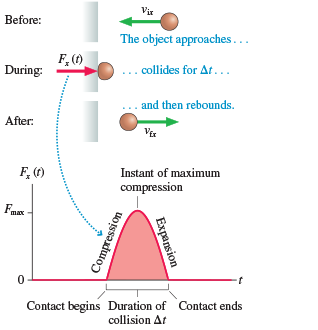
\includegraphics[width=0.6\textwidth]{../figures/collision-example.png}
    \caption{A collision.}%
    \label{fig:collision}
\end{figure}

Figure~%
\ref{fig:collision} shows an object colliding with a wall.  The object
approaches with an initial horizontal velocity
$
    v_{ix}
$%
, experience a force of duration
$
    \Delta t
$%
, and leaves with a final velocity
$
    v_{fx}
$%
.  Notice, the object is \emph{elastic} and compresses then expands,
like a spring.

The force of collision is usually very large in comparison to other
forces exerted on the object.  A large force exerted for a small
interval of time is called an \textbf{impulsive force}.  The graph in
Figure~%
\ref{fig:collision} shows how a typical impulsive force behaves.  We
write the impulsive force as
$
    F_x(t)
$%
.

We can use Newton's second law to find how the object's velocity changes
as a result of the collision.  The force at any time
$
    t
$ will be the product of the mass and the instantaneous acceleration;
thus
\begin{equation}
    ma_x=m\frac{dv_x}{dt}=F_x(t)
\end{equation}
We multiply
$
    dt
$ on both sides:
\begin{equation}
    m dv_x = F_x(t) dt
\end{equation}
The collision happens during the time interval
$
    \Delta t
$%
, so we integrate over this interval.  During this time, the velocity
changes from
$
    v_ix
$ to
$
    v_fx
$ during the collision; thus
\begin{equation}
    \label{eq:momentum-impulse-p1} m\int_{v_i}^{v_f} dv_x = mv_{fx}-mv_{ix}=\int_
    {t_i}^{t_f} F_x(t) dt
\end{equation}
To understand this equation, we need to look at momentum and impulse.

\subsection{Momentum}

\begin{definition}[Momentum]
    The product of a particle's mass and velocity.
    \begin{equation}
        \vec{p} \coloneqq m\vec{v}
    \end{equation}
\end{definition}

Looking back at Equation~%
\ref{eq:momentum-impulse-p1}, you can see that
$
    mv_{ix}
$ and
$
    mv_{fx}
$ are
$
    p_{ix}
$ and
$
    p_{fx}
$%
, the
$
    x
$-component of the particle's momentum before and after the collision.
In terms of momentum, Equation~%
\ref{eq:momentum-impulse-p1} is
\begin{equation}
    \label{eq:momentum-impulse-p2} \Delta p_x = p_{fx} - p_{ix} = \int_{t_i}^
    {t_f} F_x(t) dt
\end{equation}

\subsection{Impulse}

Equation~%
\ref{eq:momentum-impulse-p2} tells us momentum is related to the time
integral of the force.

\begin{definition}[Impulse]
    Area under
    $
        F_x(t)
    $ curve between
    $
        t_i
    $ and
    $
        t_f
    $
    \begin{equation}
        J_x \coloneqq \int_{t_i}^{t_f} F_x(t) dt
    \end{equation}
\end{definition}

Equation~%
\ref{eq:momentum-impulse-p1} can now be written as
\begin{equation}
    \Delta p_x = J_x
\end{equation}
This is called the \textbf{momentum principle}.

\subsection{Conservation of Momentum}

\begin{figure}
    \centering
    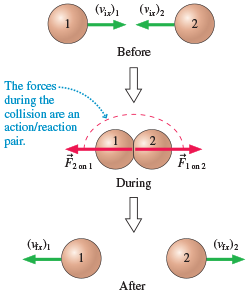
\includegraphics[width=0.4\textwidth]{../figures/two-object-collision}
    \caption{A collision between two objects}%
    \label{fig:two-object-collision}
\end{figure}

Figure~%
\ref{fig:two-object-collision} shows two objects with initial velocities
$
    (v_{ix})_1
$ and
$
    (v_{ix})_2
$%
.  The objects collide, then bounce apart with final velocities
$
    (v_{fx})_1
$ and
$
    (v_{fx})_2
$%
.  The forces during the collision, as the objects are interacting, are
an action/reaction pair
$
    \magarpair{1}{2}
$ and
$
    \magarpair{2}{1}
$%
.  For now, we'll continue to assume that the motion is one dimensional
along the
$
    x
$-axis.

Newton's second law for each object \emph{during} the collision is
\begin{align}
    \label{eq:conservation-of-momentum-p1} \frac{d(p_x)_1}{dt}&=(F_x)_{\mathrm
    {2~on~1}} \\
    \frac{d(p_x)_2}{dt}&=(F_x)_{\mathrm{1~on~2}}=-(F_x)_{\mathrm {2~on~1}}
\end{align}

Although Equation~%
\ref{eq:conservation-of-momentum-p1} are for two different objects,
suppose--just to see what happens--we were to \emph{add} these two
equations.  If we do, we find that
\begin{equation}
    \od{(p_x)_1}{t} + \od{(p_x)_2}{t} = \od{}{t}[(p_x)_1 + (p_x)_2]= (F_x)_
    {\mathrm{2~on~1}} + (-(F_x)_{\mathrm{2~on~1}}) = 0
\end{equation}

If the derivative of the quantity of
$
    (p_x)_1 + (p_x)_2
$ with respect to time is zero, it must be the case that
\begin{align}
    \label{eq:conservation-of-momentum-p2} (p_x)_1 + (p_x)_2 = \mathrm{~constant}
\end{align}
Equation~%
\ref{eq:conservation-of-momentum-p2} is a conservation law!  If
$
    (p_x)_1 + (p_x)_2
$ is a constant, then the sum of the momenta \emph{after} the collision
equals the sum of the momenta \emph{before} the collision.  That is,
\begin{align}
    \label{eq:conservation-of-momentum-p3} (p_{fx})_1 + (p_{fx})_2 = (p_
    {ix})_1 + (p_{ix})_2
\end{align}

\subsection{Systems of Particles} While Equation~%
\ref{eq:conservation-of-momentum-p3} illustrates the idea of a
conservation law of momentum, it was derived for the specific case of
two particles colliding in one dimension.  Our goal is to develop a more
general law of conservation of momentum.

\begin{figure}
    \centering
    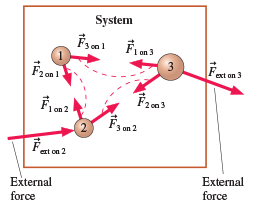
\includegraphics[width=0.4\textwidth]{../figures/n-particle-system.png}
    \caption{A system of particles}%
    \label{fig:n-particle-system}
\end{figure}

Consider a system with
$
    N
$ particles, such as the one in Figure~%
\ref{fig:n-particle-system} where
$
    N=3
$%
.  Every particle in this system \emph{interacts} with every other
particle via action/reaction pairs of forces
$
    \vec{F}_{j\on k}
$ and
$
    \vec{F}_{k\on j}
$%
.  Every particle is subjected to possible \emph{external} forces
$
    \vec{F}_{\mathrm{ext}\on k}
$%
from agents outside the system.

If particle
$
    k
$ has a velocity
$
    \vec{v}_k
$%
, its momentum is
$
    \vec{p}_k = m_k \vec{v}_k
$%
.  Let
$
    \vec{P}
$ be the \textbf{total momentum} of the system:
\begin{equation}
    \vec{P} = \sum_{k=1}^{N} \vec{p}_k
\end{equation}

The derivative of
$
    \vec{P}
$ with respect to time tells us how the total momentum changes with
time:
\begin{equation}
    \label{eq:conservation-of-momentum-p4} \od{\vec{P}}{t} = \sum_k \od{\vec
    {p}_k}{t} = \sum_k \vec{F}_k
\end{equation}
where

$
    \vec{F}_k
$ is the net force of particle at the instantaneous time
$
    \dif t
$

The net force acting on particle
$
    k
$ can be divided into \emph{external forces}, from outside the system,
and \emph{interaction forces} due to all other particles in the system:
\begin{equation}
    \vec{F}_k = \sum_{j\neq k} \vec{F}_{j \on k} + \vec{F}_{\mathrm{ext}
    \on k}
\end{equation}
where the restriction
$
    j \neq k
$ expresses that particle
$
    k
$ does not exert a force on itself.  Using this in Equation~%
\ref{eq:conservation-of-momentum-p4}
\begin{equation}
    \label{eq:conservation-of-momentum-p5} \od{\vec{P}}{t} = \sum_k \sum_
    {j \neq k} \vec{F}_{j \on k} + \vec{F}_{\mathrm{ext} \on k}
\end{equation}
The double sum on
$
    \vec{F}_{j \on k}
$ adds \emph{every} interaction force within a system.  But the
interaction forces come in action/reaction pairs, with
$
    \vec{F}_{j \on k} = -\vec{F}_{k \on j}
$ %
, so
$
    \vec{F}_{j \on k} + \vec{F}_{k \on j} = \vec{0}
$ %
.  Consequently, \textbf{the sum of all the interaction forces is zero}.
As a result, Equation~%
\ref{eq:conservation-of-momentum-p5} becomes
\begin{equation}
    \label{eq:conservation-of-momentum-p6} \od{\vec{P}}{t} = \vec{F}_ {\mathrm
    {ext} \on k} = \fnet
\end{equation}

Equation~%
\ref{eq:conservation-of-momentum-p6} has two important implications.
First, we can analzye the motion of a system as a whole without needing
to consider interactions between particles that make up the system.
When we draw particle models, we assume that the internal forces between
the atoms--forces that hold the object together--do not afftect the
motion of the object.  Now we have \emph{justified} that assumption.

\subsection{Isolated Systems}

\begin{definition}[Isolated System]
    A system that is not influenced or altered by external forces from
    the enviroment
\end{definition}

The second implication of Equation~%
\ref{eq:conservation-of-momentum-p6} applies to an isolated system.  For
momentum, that means a system on which the \emph{net} external force is
zero.

For an isolated system, Equation~%
\ref{eq:conservation-of-momentum-p6} is simply
\begin{equation}
    \od{\vec{P}}{t} = \vec{0}
\end{equation}
I.e., \textbf{the total momentum of an isolated system does not change}.

\begin{theorem}[Law of conservation of momentum]
    The total momentum
    $
        \vec{P}
    $ of an isolated system does not change.  Interactions within the
    system does not change the system's total momentum
    \begin{equation}
        \label{eq:law-of-conservation-of-momentum} \vec{P}_\fin = \vec{P}_\ini
    \end{equation}
\end{theorem}
The total momentum \emph{after} an interaction is equal to the total
momentum \emph{before} an interaction.  Because Equation~%
\ref{eq:law-of-conservation-of-momentum} is a vector equation, the
equality is true for each of the components of the momentum vecotr. That
is,
\begin{align}
    \sum_k^N (p_{\fin x})_k &= \sum_k^N (p_{\ini x})_k \\
    \sum_k^N (p_{\fin y})_k &= \sum_k^N (p_{\ini y})_k
\end{align}
\begin{remark}
    It is worth mentioning the critical role of Newton's third law.  The
    law of conservation of momentum is a direct consequence of the fact
    interactions within an isolated system are action/reaction pairs.
\end{remark}

\begin{Exercise}[title={A glider collision}, origin={Knight}]
    A \SI{250}{\gram} air-track glider is pushed across a level track at
    \SI{0.75}{\metre\per\second} toward a \SI{500}{\gram} glider that is
    at rest and bounces back at \SI{0.21}{\metre\per\second}.  What is
    the speed of the \SI{500}{\gram} glider after the collision?
\end{Exercise}

\begin{Answer}
    Let our system be the \SI{200}{\gram} glider and the \SI{500}{\gram}
    glider.  This is an isolated system.  Knowing that in an isolated
    system, interactions within the system does not change the system's
    total momentum.  Thus, for any object
    $
        k
    $ in the system,
    \begin{equation}
        \sum_k^N (p_{\fin x})_k = \sum_k^N (p_{\ini x})_k
    \end{equation}
    Knowing that the total momentum in a isolated system at one time is
    the same as the total momentum at another time,
    \begin{equation}
        m_1(v_{\fin x})_1 + m_2(v_{\fin x})_2 = m_1(v_{\ini x})_1 + m_2(v_
        {\ini x})_2
    \end{equation}
    where the \SI{200}{\gram} glider is labeled 1, and the \SI{500}{\gram}
    glider is labeled 2.  Now we solve for the velocity of glider 2
    after the collision:
    \begin{align}
        m_2(v_{\fin x})_2 &= m_1(v_{\ini x})_1 + m_2(v_{\ini x})_2 - m_1
        (v_{\fin x})_1 \\
        (v_{\fin x})_2 &= \frac{m_1(v_{\ini x})_1 + m_2(v_ {\ini x})_2 -
        m_1(v_{\fin x})_1}{m_2} \\
        &=\frac{m_1}{m_2}[(v_{\ini x})_1 - (v_{\fin x})_1] + (v_{\ini x})_2
        \\
        &=\qty{0.48}{\metre\per\second}
    \end{align}
\end{Answer}

\subsection{Inelastic Collisions}

\begin{definition}[Perfectly Inelastic Collision]
    A collision in which two objects stick together and move with a
    common final velocity
\end{definition}

As Figure~%
\ref{fig:inelastic-collision} shows, the key to analyzing a perfectly
inelastic collision is the fact that \textbf{common final velocity}.

\begin{figure}
    \centering
    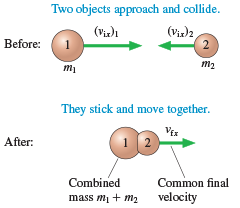
\includegraphics[width=0.4\textwidth]{../figures/an-inelastic-collision.png}
    \caption{An inelastic collision.}%
    \label{fig:inelastic-collision}
\end{figure}

\subsection{Explosions}

\begin{definition}[Explosion]
    An explosion, where the particles of a system move apart from each
    other after a brief, intense interaction, is the opposite of a
    collision.
\end{definition}

If the system is isolated, its total momentum during an explosion will
be conserved.

\begin{Exercise}[title={Recoil}, origin={Knight}]
    A \SI{10}{\gram} bullet is fired from a \SI{3.0}{\kilogram} rifle
    with a speed of \SI{500}{\metre\per\second}.  What is the recoil
    speed of the rifle?
\end{Exercise}

\begin{Answer}
    The rifle causes a small mass of gunpowder to explode, and the
    expanding gas then exerts force on \emph{both} the bullet and the
    rifle.  We will define the system to be the bullet, gas, and rifle.

    The
    $
        x
    $-component of the total momentum is
    $
        P_x=(p_x)_B + (p_x)_R + (p_x)_G
    $%
.    Everything is at rest before the trigger is pulled, so the initial
    momentum is zero.  After the trigger is pulled, the momentum of the
    expanding gas is the sum of the momenta of all the molecules in the
    gas.  For every molecule moving in the forward direction with
    velocity
    $
        v
    $ and momentum
    $
        mv
    $ there is, on average, another molecule moving in the opposite
    direction with velocity
    $
        -v
    $ and momentum
    $
        -mv
    $%
.    Thus, we will be left with
    $
        (p_x)_G \approx 0
    $%
    .
\end{Answer}
